\documentclass[10pt]{article}
\usepackage[ngerman]{babel}
\usepackage[utf8]{inputenc}
\usepackage[T1]{fontenc}
\usepackage{amsmath}
\usepackage{amsfonts}
\usepackage{amssymb}
\usepackage[version=4]{mhchem}
\usepackage{stmaryrd}
\usepackage{graphicx}
\usepackage[export]{adjustbox}
\graphicspath{ {./images/} }

\title{Hauptprüfung Abiturprüfung 2024 - Leistungsfach }

\author{Alexander Schwarz\\
www.mathe-aufgaben.com}
\date{}


\begin{document}
\maketitle
 Baden-Württemberg

\section*{Aufgabe I 2.1}
Zur Untersuchung der Lungenfunktion muss eine Person tief einatmen und anschließend zügig in ein Messgerät ausatmen. Die Änderungsrate des Luftvolumens pro Zeiteinheit beim Ausatmen heißt Atemfluss. Bei einer Messung wird der Atemfluss für $0 \leq t \leq 2$ näherungsweise durch die Funktion $f$ mit $f(t)=30 \cdot\left(e^{-3 t}-e^{-6 t}\right)$ beschrieben (t in Sekunden seit Beginn des Ausatmens, $f(t)$ in Liter pro Sekunde). Abgebildet ist der Graph von f. Für die Ableitungsfunktion f' von $f$ gilt $f^{\prime}(t)=-90 e^{-3 t} \cdot\left(1-2 e^{-3 t}\right)$.\\
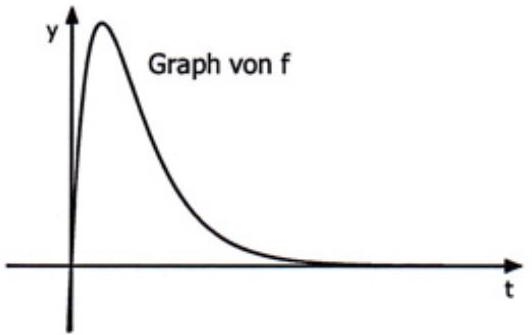
\includegraphics[max width=\textwidth, center]{2025_04_24_b51c588d66752015e66cg-2}\\
a) Weisen Sie nach, dass der maximale Atemfluss 7,5 Liter pro Sekunde beträgt.\\
(4 BE)\\
b) Zeigen Sie, dass der Atemfluss zwei Sekunden nach Beginn des Ausatmens weniger als ein Prozent seines maximalen Werts beträgt.\\
(2 BE)\\
c) Bestimmen Sie rechnerisch die Länge des Zeitraums, in dem der Atemfluss mindestens 5 Liter pro Sekunde beträgt.\\
(7 BE)\\
d) Formulieren Sie eine Fragestellung im Sachzusammenhang, die auf die Gleichung $\int_{0}^{x} f(t) d t=\frac{1}{4} \cdot \int_{0}^{2} f(t) d t$ führt.\\
e) Berechnen Sie $\int_{0}^{2} f(t) d t$.\\
f) Bei einer anderen Modellierung wird der Atemfluss ab dem Zeitpunkt $\mathrm{t}_{1}=1,5$ nicht mehr durch die Funktion f, sondern durch die Gleichung der Tangente an den Graphen von $f$ im Punkt $P(1,5 \mid f(1,5))$ beschrieben. Bei dieser Modellierung gibt es einen Zeitpunkt $t_{2}>0$, zu dem der Atemfluss 0 Liter pro Sekunde beträgt. Bestimmen Sie den Wert von $\mathrm{t}_{2}$.\\
g) Bei ärztlichen Untersuchungen werden Atemfluss-Volumen-Diagramme betrachtet. Diese stellen den Atemfluss in Abhängigkeit vom Volumen der ausgeatmeten Luft dar. Abgebildet ist das Diagramm zu derjenigen Messung, die durch die Funktion $f$ beschrieben wird.\\
Betrachtet wird der Hochpunkt $\mathrm{H}\left(\mathrm{x}_{0} \mid \mathrm{y}_{0}\right)$ der abgebildeten Kurve. Begründen Sie, dass $y_{0}$ der in a) genannte maximale Atemfluss ist, und geben Sie einen Term an, mit dem man $\mathrm{x}_{0}$ berechnen kann.\\
(4 BE)\\
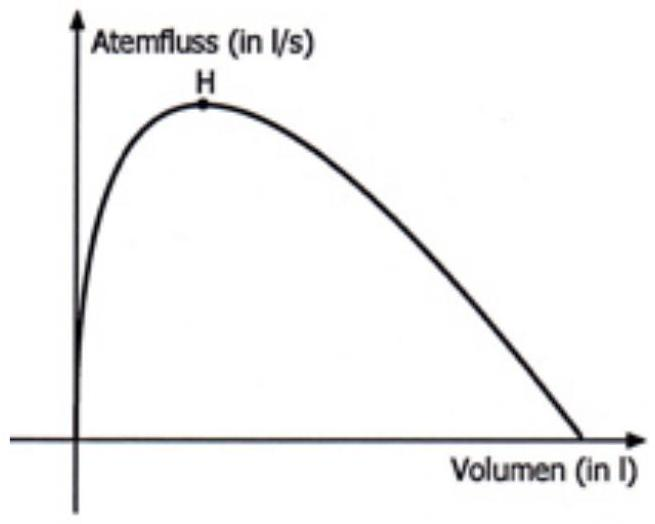
\includegraphics[max width=\textwidth, center]{2025_04_24_b51c588d66752015e66cg-3}

\section*{Aufgabe I 2.2}
Für jedes a mit $0<a<1$ ist eine Funktion $f_{a}$ mit $f_{a}(x)=(x-2)^{3}+a(x-2)+2$ gegeben.\\
a) Weisen Sie nach, dass jede Funktion $f_{a}$ streng monoton wachsend ist. (4 BE)

Die Tangente $t_{a}$ an den Graphen von $f_{a}$ im Punkt $P(2 \mid 2)$, die Tangente an den Graphen der Umkehrfunktion $\overline{f_{a}}$ im Punkt $P$ und die Koordinatenachsen schließen im 1.Quadranten des Koordinatensystems ein Viereck $V_{a}$ ein. $Q_{a}$ ist der Schnittpunkt von $t_{a}$ mit der $y$-Achse. Abgebildet sind beispielhaft der Graph von $f_{0,25}$ sowie die Tangente $\mathrm{t}_{0,25}$.\\
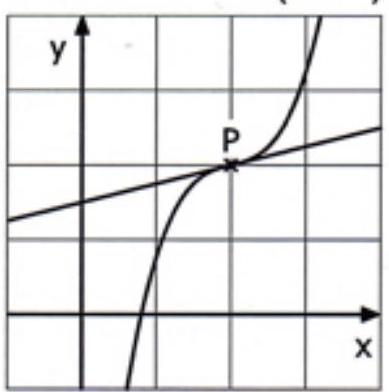
\includegraphics[max width=\textwidth, center]{2025_04_24_b51c588d66752015e66cg-3(1)}\\
b) Begründen Sie, dass der Punkt $\mathrm{Q}_{\mathrm{a}}$ zwischen dem Ursprung und dem Punkt (0|2) liegt und dass der Flächeninhalt des Vierecks $V_{a}$ kleiner als 4 ist.\\
c) Für einen Wert von a hat der Innenwinkel des Vierecks $V_{a}$ bei $P$ die Größe $60^{\circ}$. Begründen Sie ohne Berechnung des Werts von a, dass der Steigungswinkel der zugehörigen Tangente $t_{a}$ die Größe $15^{\circ}$ hat.\\
(3 BE)

\section*{Lösungen}
\section*{Aufgabe I 2.1}
a) Notwendige Bedingung für eine Maximumstelle: $f^{\prime}(t)=0$\\
$-90 e^{-3 t} \cdot\left(1-2 e^{-3 t}\right)=0$ Lösung mit dem Satz vom Nullprodukt\\
Gleichung I): $-90 \mathrm{e}^{-3 \mathrm{t}}=0$ ist nicht lösbar\\
Gleichung II): $1-2 \mathrm{e}^{-3 \mathrm{t}}=0 \Leftrightarrow \mathrm{e}^{-3 \mathrm{t}}=\frac{1}{2} \Leftrightarrow \mathrm{t}_{0}=-\frac{1}{3} \cdot \ln \left(\frac{1}{2}\right) \approx 0,23$\\
An der Abbildung erkennt man, dass bei $t_{0}$ eine Maximumstelle existiert.\\
Es gilt $f\left(\mathrm{t}_{0}\right)=7,5$.\\
Damit ist gezeigt, dass der maximale Atemfluss 7,5 Liter pro Sekunde beträgt.\\
b) Es gilt $f(2) \approx 0,074$.

1 Prozent von 7,5 ist $0,01 \cdot 7,5=0,075$.\\
Damit ist $f(2)<0,075$ was zu zeigen war.\\
c) Bedingung: $f(t)>5$

Zunächst wird berechnet, zu welchen Zeitpunkten der Atemfluss exakt 5 Liter pro Sekunde beträgt.\\
$f(t)=5 \Leftrightarrow 30 \cdot\left(e^{-3 t}-e^{-6 t}\right)=5 \Leftrightarrow e^{-3 t}-e^{6 t}-\frac{1}{6}=0$\\
Lösung mit Substitution $u=e^{-3 t}$\\
$u-u^{2}-\frac{1}{6}=0 \Leftrightarrow-u^{2}+u-\frac{1}{6}=0$\\
$u_{1,2}=\frac{-1 \pm \sqrt{1^{2}-4 \cdot(-1) \cdot\left(-\frac{1}{6}\right)}}{-2}=\frac{-1 \pm \sqrt{\frac{1}{3}}}{-2} \quad u_{1} \approx 0,211$ und $u_{2} \approx 0,789$\\
Rücksubstitution: $\mathrm{e}^{-3 \mathrm{t}}=0,211 \Leftrightarrow \mathrm{t} \approx-\frac{1}{3} \ln (0,211) \approx 0,52$

$$
\mathrm{e}^{-3 \mathrm{t}}=0,789 \Leftrightarrow \mathrm{t} \approx-\frac{1}{3} \ln (0,789) \approx 0,08
$$

Aus der Abbildung ergibt sich dass $f(t)>5$ gilt für $0,08<t<0,52$.\\
Die Länge des Zeitraums beträgt etwa 0,44 Sekunden.\\
d) $\int_{0}^{2} f(t) d t$ beschreibt die Menge der ausgeatmeten Luft (in Liter) in den ersten 2 Sekunden.\\
$\int_{0}^{x} f(t) d t$ beschreibt die Menge der ausgeatmeten Luft (in Liter) in den ersten $x$ Sekunden.

Fragestellung: Zu welchem Zeitpunkt x beträgt das Volumen der ausgeatmeten Luft ein Viertel des Volumens der während der ersten zwei Sekunden ausgeatmeten Luft?\\
e) $\int_{0}^{2} f(t) d t=\int_{0}^{2} 30 \cdot\left(e^{-3 t}-e^{-6 t}\right) d t=30 \cdot\left[-\frac{1}{3} e^{-3 t}+\frac{1}{6} e^{-6 t}\right]_{0}^{2} \approx-0,025-(-5)=4,975$\\
f) Allgemeine Tangentengleichung an der Stelle $t=1,5: y=f^{\prime}(1,5) \cdot(t-1,5)+f(1,5)$

Es gilt $\mathrm{f}(1,5) \approx 0,33$ und $\mathrm{f}^{\prime}(1,5) \approx-0,98$\\
Tangentengleichung: $y=-0,98 \cdot(t-1,5)+0,33 \Leftrightarrow y=-0,98 t+1,8$\\
Schnittstelle der Tangente mit der t-Achse: $0=-0,98 t+1,8 \Leftrightarrow t \approx 1,84$\\
Der gesuchte Zeitpunkt beträgt $\mathrm{t}_{2} \approx 1,84$ Sekunden\\
g) Begründen Sie, dass $y_{0}$ der in a) genannte maximale Atemfluss ist.

Der maximale Atemfluss beträgt gemäß a) 7,5 Liter pro Sekunde (dies entspricht der Einheit auf der y-Achse der Abbildung). Hierbei spielt es keine Rolle ob auf der x-Achse die Zeit in Sekunden oder das ausgeatmete Volumen abgetragen ist.

Geben Sie einen Term an, mit dem man $\mathrm{x}_{0}$ berechnen kann.\\
$\mathrm{x}_{0}$ entspricht der Menge der ausgeatmeten Luft bis zum Zeitpunkt\\
$\mathrm{t}_{0}=-\frac{1}{3} \cdot \ln \left(\frac{1}{2}\right)$.\\
$x_{0}=\int_{0}^{t_{0}} f(t) d t$

\section*{Aufgabe I 2.2}
a) Es gilt $f_{a}^{\prime}(x)=3 \cdot(x-2)^{2}+a$

Da a $>0$ ist und $(x-2)^{2} \geq 0$ ist gilt $f_{a}^{\prime}(x)>0$.\\
Somit ist $\mathrm{f}_{\mathrm{a}}$ streng monoton wachsend.\\
b) Begründen Sie, dass der Punkt $\mathrm{Q}_{\mathrm{a}}$ zwischen dem Ursprung und dem Punkt (0|2) liegt.

Es gilt $f_{a}^{\prime}(2)=$ a mit $0<a<1$.\\
Da die Tangentensteigung positiv ist, liegt der Punkt $Q_{a}$ unterhalb von $P$.\\
Damit liegt $\mathrm{Q}_{\mathrm{a}}$ unterhalb von $\mathrm{B}(0 \mid 2)$.\\
Da die Steigung kleiner als 1 ist, liegt $Q_{a}$ oberhalb des Ursprungs $O(0 \mid 0)$.\\
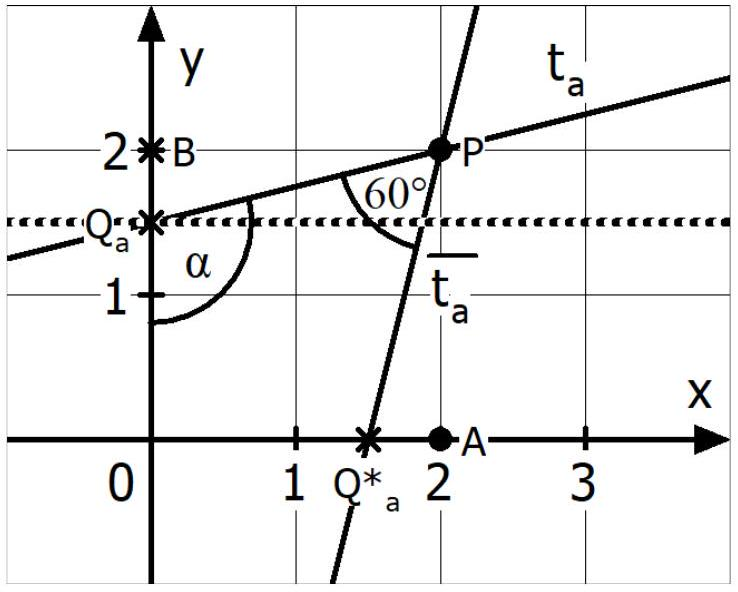
\includegraphics[max width=\textwidth, center]{2025_04_24_b51c588d66752015e66cg-6}

Begründen Sie, dass der Flächeninhalt des Vierecks $\mathrm{V}_{\mathrm{a}}$ kleiner als 4 ist.\\
Die Gerade $\overline{t_{a}}$ ist die Tangente in $P$ an das Schaubild der Umkehrfunktion $\overline{f_{a}}$.\\
Der Schnittpunkt $Q_{a}^{*}$ von $\overline{\mathrm{t}_{\mathrm{a}}}$ mit der x-Achse liegt aus Symmetriegründen analog zu $Q_{a}$ zwischen dem Punkt $O(0 \mid 0)$ und $A(2 \mid 0)$.

Das Viereck $\mathrm{V}_{\mathrm{a}}$ mit den Eckpunkten $\mathrm{OQ}_{\mathrm{a}} \mathrm{PQ}_{\mathrm{a}}$ liegt innerhalb der Quadrats OAPB, das den Flächeninhalt 4 besitzt.\\
Somit hat $\mathrm{V}_{\mathrm{a}}$ einen Flächeninhalt, der kleiner ist als 4.\\
c) Der Winkel bei $P$ sei $60^{\circ}$ und der Winkel bei $O(0 \mid 0)$ beträgt $90^{\circ}$.

Die Winkel in den Punkten $Q_{a}$ und $Q_{a}^{*}$ sind gleich groß aufgrund der Symmetrie.\\
Daher gilt aufgrund der Winkelsumme im Viereck $\alpha=\frac{360^{\circ}-60^{\circ}-90^{\circ}}{2}=105^{\circ}$.\\
Der obere Teil des Winkels $\alpha$ zwischen der gestrichelten waagrechten Gerade und der Tangente $t_{a}$ ist der Steigungswinkel der Tangente.\\
Dieser beträgt $105^{\circ}-90^{\circ}=15^{\circ}$ was zu zeigen war.


\end{document}